%=============================================================================
%  CHAPTER 1 — PROJECT FRAMEWORK
%=============================================================================
\chapter{Project Framework}

\clearpage
\section*{Introduction}

Before describing the technical work carried out on ForsaDrive, it is necessary to situate the project in its concrete context. This chapter therefore presents the host organization within which the internship was conducted, examines the current state of mobility in Tunisia and the limits of the solutions that users currently rely on, and finally states the motivations and objectives that led to the development of the platform. The chapter closes with an outline of the proposed solution, which serves as the bridge towards the analysis of requirements presented in the next chapter.


\section{Study of the Host Organization}

\subsection{Presentation of ATOMIC IT}

ATOMIC IT is an information technology engineering services company specialized in the design and development of digital solutions. Its team brings together engineers, technicians, and IT specialists who work primarily on web and mobile development. The company assists its clients in the full lifecycle of their software projects, from the initial expression of needs to the deployment and maintenance of the delivered system.

Beyond pure development, ATOMIC IT positions itself as a partner that helps its clients translate business requirements into reliable digital tools. It relies on modern technologies and on programming environments such as Windows and Linux, the .NET and Java ecosystems, and the major mobile platforms (Android and iOS). This breadth of expertise allows the company to work on a wide range of projects, from institutional websites to platforms with significant business logic such as the one developed during this internship.

\subsection{General Information about ATOMIC IT}

Table~\ref{tab:atomic_info} summarizes the main administrative information about the host organization.

\begin{table}[H]
\centering
\caption{General information about ATOMIC IT}
\label{tab:atomic_info}
\begin{tabular}{|l|p{9cm}|}
\hline
\textbf{Address}      & Arab League Street, Kélibia, Nabeul Governorate \\
\hline
\textbf{Phone Number} & +216 55 343 224 \\
\hline
\textbf{Activity}     & Web and mobile development, software engineering, and digital consulting \\
\hline
\textbf{Director}     & Mr. Khalil Selmi \\
\hline
\textbf{Core focus}   & Design and delivery of responsive web platforms and mobile applications adapted to client needs \\
\hline
\end{tabular}
\end{table}

\subsection{Services Offered by ATOMIC IT}

The company structures its activity around four main services that complement each other.

\begin{description}[noitemsep]
    \item[Website Creation.] Design of responsive and customized websites, with attention to performance, accessibility, and scalability. The company adapts the technical stack to the client's profile, whether the goal is a content-driven site or a more dynamic interface.
    \item[Web Engineering.] Development of more complex platforms such as e-commerce systems, community platforms, and data-driven applications. This service covers backend architecture, database modeling, and the integration of third-party components such as payment gateways or notification services.
    \item[Web Marketing.] Support in the definition of digital marketing strategies. The company assists its clients in the choice of channels, the structuring of campaigns, and the alignment of online communication with measurable business objectives.
    \item[Search Engine Optimization.] Improvement of the visibility of websites in search engines through keyword strategies, indexing, and the application of best practices in technical and content SEO.
\end{description}

The internship took place primarily within the engineering activity of the company, since ForsaDrive belongs to the family of data-driven platforms with significant business logic.

\subsection{Organizational Chart of ATOMIC IT}

The internal organization of ATOMIC IT is deliberately flat and oriented towards short communication paths between decision making and execution. Figure~\ref{fig:atomic_org} presents the simplified organizational chart of the company.

\begin{figure}[H]
    \centering
    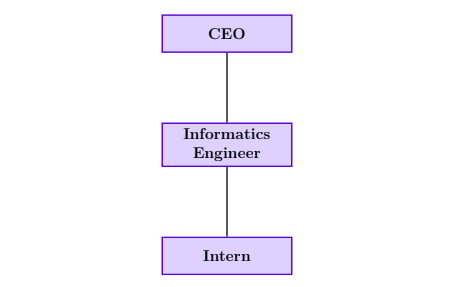
\includegraphics[width=0.8\textwidth]{image.png}
    \caption{Organizational chart of ATOMIC IT}
    \label{fig:atomic_org}
\end{figure}

At the top level, the chief executive officer supervises strategic decisions, validates project directions, and represents the company with its clients. The development teams handle the technical implementation, while interns contribute to ongoing projects under the supervision of senior developers. This structure favors quick feedback loops, which proved beneficial during the internship since the validation of design choices on ForsaDrive could take place without intermediate delays.

\subsection{Internship Framework}

The internship was carried out within the development team of the company, in coordination with both frontend and backend developers. The work followed an agile Scrum approach, with daily stand-up meetings inside the team and weekly reviews with the supervising engineer. This rhythm allowed a continuous validation of progress and gave the opportunity to adjust priorities as the project advanced.

The two interns who collaborated on ForsaDrive worked on the same shared application rather than on two independent products. The work was therefore distributed by functional modules and by sprints, not by a strict separation between web and mobile responsibilities. This organization made it possible to keep the business logic consistent across the two interfaces and to share the design effort on the most sensitive parts of the system, such as authentication, the booking flow, and the payment logic.


\section{Critical Study of the Existing Situation}

\subsection{General Context}

Mobility plays a central role in economic activity, education, and social interaction. In Tunisia, transportation conditions every aspect of daily life, from the choice of a university to the feasibility of a job offer in another governorate. Yet, the available means of transportation suffer from structural limitations that make travel both expensive and unpredictable. Public transport between cities is often overcrowded and irregular, the road network does not always serve secondary towns with the same frequency as the main corridors, and private cars travel every day with empty seats that no system currently helps to fill.

This situation places a particular burden on students and young professionals, who travel frequently but have limited budgets. It is in this segment that the demand for a reliable and affordable shared mobility service is the most visible.

\subsection{Analysis of Current Limitations}

The mobility solutions currently available in Tunisia each address part of the problem but leave significant gaps. Public transport remains the cheapest option, but its capacity is limited and its schedule does not match the flexibility that students or workers often need. Informal carpooling, which is mostly organized through Facebook groups and private messaging, fills part of the demand but does so without any structure: there is no verification of the identity of drivers or vehicles, no traceability of payments, no centralized search, and no mechanism to rate or report a user after a trip. International applications such as Bolt or inDrive operate on a ride-hailing model designed for short urban trips, and their pricing logic is not adapted to long-distance carpooling. International carpooling platforms such as BlaBlaCar are technically suitable but suffer from a low local adoption, partly because their payment methods, customer support, and user base are not aligned with the realities of the Tunisian market.

Several recurring weaknesses can be summarized as follows:

\begin{itemize}[noitemsep]
    \item Public transport suffers from delays, overcrowding, and insufficient geographic coverage.
    \item Existing international platforms are not fully adapted to local realities such as payment methods, identity verification, or regional mobility patterns.
    \item Informal ride-sharing lacks trust mechanisms such as identity checks, ratings, or secure communication channels.
    \item Private vehicles are underutilized, with many empty seats during daily and weekly trips.
    \item No centralized solution offers a structured advantage to students, who form a large part of the inter-city travel demand.
\end{itemize}

These limitations highlight the absence of a structured, secure, and locally adapted system for shared mobility.

\subsection{Problem Statement}

The analysis of the existing situation can be condensed into a single observation:

\begin{quote}
\textit{Tunisia lacks a secure, affordable, and well-structured digital ride-sharing solution that is adapted to local payment habits, available on both web and mobile, and capable of building genuine trust between drivers and passengers.}
\end{quote}

The challenge is therefore not to invent a new concept, but to adapt the proven model of carpooling to the specific constraints of the Tunisian context.

\subsection{Project Motivation}

The motivation behind ForsaDrive is at the same time social, economic, and technical. On the social side, the project aims to make mobility more accessible to populations whose budget excludes private taxis and whose schedule is not always compatible with public transport, particularly students. On the economic side, the platform contributes to a better use of an existing resource, namely the empty seats of vehicles already on the road, which translates into shared savings for drivers and passengers. On the technical side, the project offers the opportunity to design a complete software ecosystem, articulating a web application, a mobile application, and a shared backend around a coherent business logic.

\subsection{Project Objectives}

The general objective of the project is the design and the implementation of a complete carpooling platform adapted to the Tunisian context. This general objective is broken down into the following specific objectives:

\begin{enumerate}[noitemsep]
    \item Develop a web platform that supports the management of rides and the administration of the system.
    \item Build a mobile application that covers the daily interactions of drivers and passengers.
    \item Provide a unified backend that exposes a single set of business rules to both clients.
    \item Integrate trust mechanisms based on identity verification, ratings, and complaint handling.
    \item Implement a wallet-based payment flow with a fifty-percent prepayment that confirms the booking and a remaining balance settled in cash during the trip.
    \item Offer a verified student status that grants an automatic discount on eligible trips.
    \item Ensure security, scalability, and maintainability throughout the architecture.
\end{enumerate}

\subsection{Proposed Solution}

ForsaDrive is designed as an integrated ecosystem composed of three coordinated components: a web application, a mobile application, and a shared backend. The platform supports the complete carpooling lifecycle, from registration to post-trip evaluation. A driver can publish a trip with its origin, destination, date, price, and number of available seats. A passenger can search for trips, filter results, consult the profile of the driver, book one or several seats, and confirm the booking through a fifty-percent prepayment. After the trip, both parties can rate each other, and any incident can be reported to the administration through a dedicated complaint channel.

The originality of the platform lies in the careful adaptation of every feature to the local context: the payment flow combines an online prepayment with a cash settlement, in line with the way Tunisian users currently handle informal carpooling; the student status is verified through documents or a university email, which makes the discount both accessible and auditable; and the interface is designed to support the languages effectively used by the target population. These choices, which are detailed in the following chapters, are what distinguish ForsaDrive from the international platforms that have so far failed to gain a strong foothold in the country.


\section*{Conclusion}

This chapter introduced the host organization, presented the structural limits of the current transportation situation in Tunisia, and stated the motivations that led to the development of ForsaDrive. It also formulated the general and specific objectives of the project and outlined the proposed solution at a high level. The next chapter translates this general framework into a precise specification: it analyzes the existing competing solutions in more detail, formalizes the actors of the system, and lists the functional and non-functional requirements that the platform must fulfill.